\documentclass[1p]{elsarticle_modified}
%\bibliographystyle{elsarticle-num}

%\usepackage[colorlinks]{hyperref}
%\usepackage{abbrmath_seonhwa} %\Abb, \Ascr, \Acal ,\Abf, \Afrak
\usepackage{amsfonts}
\usepackage{amssymb}
\usepackage{amsmath}
\usepackage{amsthm}
\usepackage{scalefnt}
\usepackage{amsbsy}
\usepackage{kotex}
\usepackage{caption}
\usepackage{subfig}
\usepackage{color}
\usepackage{graphicx}
\usepackage{xcolor} %% white, black, red, green, blue, cyan, magenta, yellow
\usepackage{float}
\usepackage{setspace}
\usepackage{hyperref}

\usepackage{tikz}
\usetikzlibrary{arrows}

\usepackage{multirow}
\usepackage{array} % fixed length table
\usepackage{hhline}

%%%%%%%%%%%%%%%%%%%%%
\makeatletter
\renewcommand*\env@matrix[1][\arraystretch]{%
	\edef\arraystretch{#1}%
	\hskip -\arraycolsep
	\let\@ifnextchar\new@ifnextchar
	\array{*\c@MaxMatrixCols c}}
\makeatother %https://tex.stackexchange.com/questions/14071/how-can-i-increase-the-line-spacing-in-a-matrix
%%%%%%%%%%%%%%%

\usepackage[normalem]{ulem}

\newcommand{\msout}[1]{\ifmmode\text{\sout{\ensuremath{#1}}}\else\sout{#1}\fi}
%SOURCE: \msout is \stkout macro in https://tex.stackexchange.com/questions/20609/strikeout-in-math-mode

\newcommand{\cancel}[1]{
	\ifmmode
	{\color{red}\msout{#1}}
	\else
	{\color{red}\sout{#1}}
	\fi
}

\newcommand{\add}[1]{
	{\color{blue}\uwave{#1}}
}

\newcommand{\replace}[2]{
	\ifmmode
	{\color{red}\msout{#1}}{\color{blue}\uwave{#2}}
	\else
	{\color{red}\sout{#1}}{\color{blue}\uwave{#2}}
	\fi
}

\newcommand{\Sol}{\mathcal{S}} %segment
\newcommand{\D}{D} %diagram
\newcommand{\A}{\mathcal{A}} %arc


%%%%%%%%%%%%%%%%%%%%%%%%%%%%%5 test

\def\sl{\operatorname{\textup{SL}}(2,\Cbb)}
\def\psl{\operatorname{\textup{PSL}}(2,\Cbb)}
\def\quan{\mkern 1mu \triangleright \mkern 1mu}

\theoremstyle{definition}
\newtheorem{thm}{Theorem}[section]
\newtheorem{prop}[thm]{Proposition}
\newtheorem{lem}[thm]{Lemma}
\newtheorem{ques}[thm]{Question}
\newtheorem{cor}[thm]{Corollary}
\newtheorem{defn}[thm]{Definition}
\newtheorem{exam}[thm]{Example}
\newtheorem{rmk}[thm]{Remark}
\newtheorem{alg}[thm]{Algorithm}

\newcommand{\I}{\sqrt{-1}}
\begin{document}

%\begin{frontmatter}
%
%\title{Boundary parabolic representations of knots up to 8 crossings}
%
%%% Group authors per affiliation:
%\author{Yunhi Cho} 
%\address{Department of Mathematics, University of Seoul, Seoul, Korea}
%\ead{yhcho@uos.ac.kr}
%
%
%\author{Seonhwa Kim} %\fnref{s_kim}}
%\address{Center for Geometry and Physics, Institute for Basic Science, Pohang, 37673, Korea}
%\ead{ryeona17@ibs.re.kr}
%
%\author{Hyuk Kim}
%\address{Department of Mathematical Sciences, Seoul National University, Seoul 08826, Korea}
%\ead{hyukkim@snu.ac.kr}
%
%\author{Seokbeom Yoon}
%\address{Department of Mathematical Sciences, Seoul National University, Seoul, 08826,  Korea}
%\ead{sbyoon15@snu.ac.kr}
%
%\begin{abstract}
%We find all boundary parabolic representation of knots up to 8 crossings.
%
%\end{abstract}
%\begin{keyword}
%    \MSC[2010] 57M25 
%\end{keyword}
%
%\end{frontmatter}

%\linenumbers
%\tableofcontents
%
\newcommand\colored[1]{\textcolor{white}{\rule[-0.35ex]{0.8em}{1.4ex}}\kern-0.8em\color{red} #1}%
%\newcommand\colored[1]{\textcolor{white}{ #1}\kern-2.17ex	\textcolor{white}{ #1}\kern-1.81ex	\textcolor{white}{ #1}\kern-2.15ex\color{red}#1	}

{\Large $\underline{12n_{0339}~(K12n_{0339})}$}

\setlength{\tabcolsep}{10pt}
\renewcommand{\arraystretch}{1.6}
\vspace{1cm}\begin{tabular}{m{100pt}>{\centering\arraybackslash}m{274pt}}
\multirow{5}{120pt}{
	\centering
	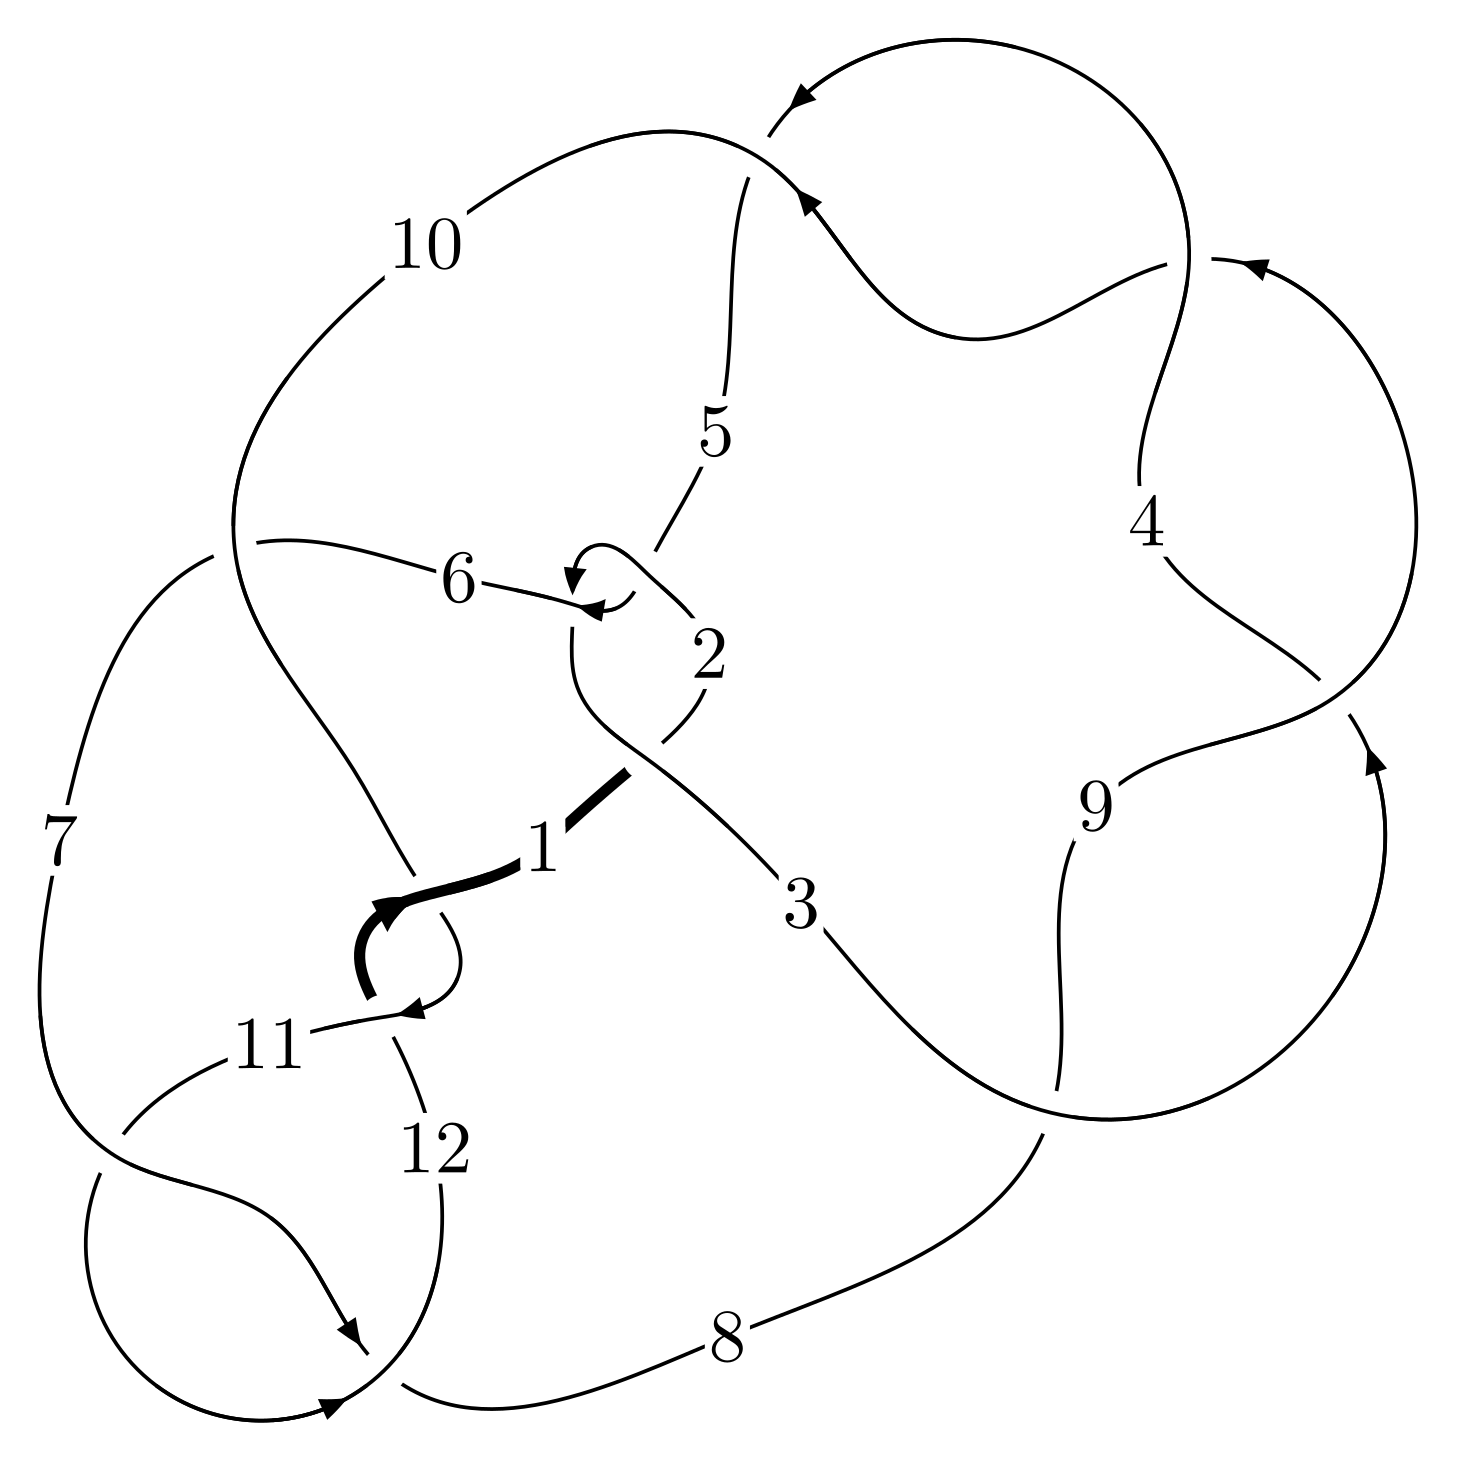
\includegraphics[width=112pt]{../../../GIT/diagram.site/Diagrams/png/2428_12n_0339.png}\\
\ \ \ A knot diagram\footnotemark}&
\allowdisplaybreaks
\textbf{Linearized knot diagam} \\
\cline{2-2}
 &
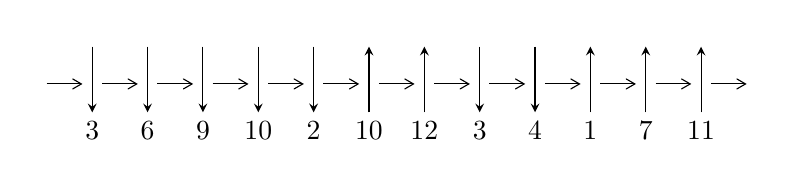
\begin{tikzpicture}[x=20pt, y=17pt]
	% nodes
	\node (C0) at (0, 0) {};
	\node (C1) at (1, 0) {};
	\node (C1U) at (1, +1) {};
	\node (C1D) at (1, -1) {3};

	\node (C2) at (2, 0) {};
	\node (C2U) at (2, +1) {};
	\node (C2D) at (2, -1) {6};

	\node (C3) at (3, 0) {};
	\node (C3U) at (3, +1) {};
	\node (C3D) at (3, -1) {9};

	\node (C4) at (4, 0) {};
	\node (C4U) at (4, +1) {};
	\node (C4D) at (4, -1) {10};

	\node (C5) at (5, 0) {};
	\node (C5U) at (5, +1) {};
	\node (C5D) at (5, -1) {2};

	\node (C6) at (6, 0) {};
	\node (C6U) at (6, +1) {};
	\node (C6D) at (6, -1) {10};

	\node (C7) at (7, 0) {};
	\node (C7U) at (7, +1) {};
	\node (C7D) at (7, -1) {12};

	\node (C8) at (8, 0) {};
	\node (C8U) at (8, +1) {};
	\node (C8D) at (8, -1) {3};

	\node (C9) at (9, 0) {};
	\node (C9U) at (9, +1) {};
	\node (C9D) at (9, -1) {4};

	\node (C10) at (10, 0) {};
	\node (C10U) at (10, +1) {};
	\node (C10D) at (10, -1) {1};

	\node (C11) at (11, 0) {};
	\node (C11U) at (11, +1) {};
	\node (C11D) at (11, -1) {7};

	\node (C12) at (12, 0) {};
	\node (C12U) at (12, +1) {};
	\node (C12D) at (12, -1) {11};
	\node (C13) at (13, 0) {};

	% arrows
	\draw[->,>={angle 60}]
	(C0) edge (C1) (C1) edge (C2) (C2) edge (C3) (C3) edge (C4) (C4) edge (C5) (C5) edge (C6) (C6) edge (C7) (C7) edge (C8) (C8) edge (C9) (C9) edge (C10) (C10) edge (C11) (C11) edge (C12) (C12) edge (C13) ;	\draw[->,>=stealth]
	(C1U) edge (C1D) (C2U) edge (C2D) (C3U) edge (C3D) (C4U) edge (C4D) (C5U) edge (C5D) (C6D) edge (C6U) (C7D) edge (C7U) (C8U) edge (C8D) (C9U) edge (C9D) (C10D) edge (C10U) (C11D) edge (C11U) (C12D) edge (C12U) ;
	\end{tikzpicture} \\
\hhline{~~} \\& 
\textbf{Solving Sequence} \\ \cline{2-2} 
 &
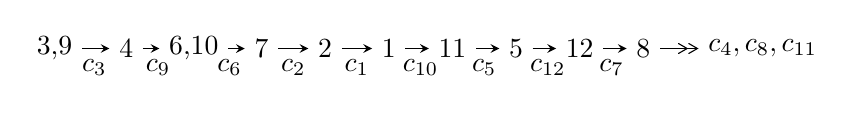
\begin{tikzpicture}[x=23pt, y=7pt]
	% node
	\node (A0) at (-1/8, 0) {3,9};
	\node (A1) at (1, 0) {4};
	\node (A2) at (33/16, 0) {6,10};
	\node (A3) at (25/8, 0) {7};
	\node (A4) at (33/8, 0) {2};
	\node (A5) at (41/8, 0) {1};
	\node (A6) at (49/8, 0) {11};
	\node (A7) at (57/8, 0) {5};
	\node (A8) at (65/8, 0) {12};
	\node (A9) at (73/8, 0) {8};
	\node (C1) at (1/2, -1) {$c_{3}$};
	\node (C2) at (3/2, -1) {$c_{9}$};
	\node (C3) at (21/8, -1) {$c_{6}$};
	\node (C4) at (29/8, -1) {$c_{2}$};
	\node (C5) at (37/8, -1) {$c_{1}$};
	\node (C6) at (45/8, -1) {$c_{10}$};
	\node (C7) at (53/8, -1) {$c_{5}$};
	\node (C8) at (61/8, -1) {$c_{12}$};
	\node (C9) at (69/8, -1) {$c_{7}$};
	\node (A10) at (11, 0) {$c_{4},c_{8},c_{11}$};

	% edge
	\draw[->,>=stealth]	
	(A0) edge (A1) (A1) edge (A2) (A2) edge (A3) (A3) edge (A4) (A4) edge (A5) (A5) edge (A6) (A6) edge (A7) (A7) edge (A8) (A8) edge (A9) ;
	\draw[->>,>={angle 60}]	
	(A9) edge (A10);
\end{tikzpicture} \\ 

\end{tabular} \\

\footnotetext{
The image of knot diagram is generated by the software ``\textbf{Draw programme}" developed by Andrew Bartholomew(\url{http://www.layer8.co.uk/maths/draw/index.htm\#Running-draw}), where we modified some parts for our purpose(\url{https://github.com/CATsTAILs/LinksPainter}).
}\phantom \\ \newline 
\centering \textbf{Ideals for irreducible components\footnotemark of $X_{\text{par}}$} 
 
\begin{align*}
I^u_{1}&=\langle 
1.66975\times10^{42} u^{55}-3.16547\times10^{41} u^{54}+\cdots+4.47134\times10^{42} b-8.10923\times10^{42},\\
\phantom{I^u_{1}}&\phantom{= \langle  }-1.22687\times10^{42} u^{55}-2.29862\times10^{42} u^{54}+\cdots+1.78854\times10^{43} a-5.42549\times10^{43},\;u^{56}+u^{55}+\cdots-24 u-8\rangle \\
I^u_{2}&=\langle 
b+1,\;4 a^3+2 a^2 u+12 a^2+4 a u+16 a+3 u+8,\;u^2-2\rangle \\
\\
I^v_{1}&=\langle 
a,\;b-1,\;v^3- v^2+2 v-1\rangle \\
\end{align*}
\raggedright * 3 irreducible components of $\dim_{\mathbb{C}}=0$, with total 65 representations.\\
\footnotetext{All coefficients of polynomials are rational numbers. But the coefficients are sometimes approximated in decimal forms when there is not enough margin.}
\newpage
\renewcommand{\arraystretch}{1}
\centering \section*{I. $I^u_{1}= \langle 1.67\times10^{42} u^{55}-3.17\times10^{41} u^{54}+\cdots+4.47\times10^{42} b-8.11\times10^{42},\;-1.23\times10^{42} u^{55}-2.30\times10^{42} u^{54}+\cdots+1.79\times10^{43} a-5.43\times10^{43},\;u^{56}+u^{55}+\cdots-24 u-8 \rangle$}
\flushleft \textbf{(i) Arc colorings}\\
\begin{tabular}{m{7pt} m{180pt} m{7pt} m{180pt} }
\flushright $a_{3}=$&$\begin{pmatrix}1\\0\end{pmatrix}$ \\
\flushright $a_{9}=$&$\begin{pmatrix}0\\u\end{pmatrix}$ \\
\flushright $a_{4}=$&$\begin{pmatrix}1\\u^2\end{pmatrix}$ \\
\flushright $a_{6}=$&$\begin{pmatrix}0.0685965 u^{55}+0.128520 u^{54}+\cdots+1.30791 u+3.03348\\-0.373433 u^{55}+0.0707946 u^{54}+\cdots+4.21694 u+1.81360\end{pmatrix}$ \\
\flushright $a_{10}=$&$\begin{pmatrix}- u\\- u^3+u\end{pmatrix}$ \\
\flushright $a_{7}=$&$\begin{pmatrix}-0.405753 u^{55}+0.122299 u^{54}+\cdots+7.07171 u+5.59685\\-0.513211 u^{55}+0.0509245 u^{54}+\cdots+5.89345 u+2.99527\end{pmatrix}$ \\
\flushright $a_{2}=$&$\begin{pmatrix}-0.240787 u^{55}+0.0796338 u^{54}+\cdots+3.53793 u+4.36769\\-0.164966 u^{55}+0.0426655 u^{54}+\cdots+3.53379 u+1.22915\end{pmatrix}$ \\
\flushright $a_{1}=$&$\begin{pmatrix}-0.405753 u^{55}+0.122299 u^{54}+\cdots+7.07171 u+5.59685\\-0.164966 u^{55}+0.0426655 u^{54}+\cdots+3.53379 u+1.22915\end{pmatrix}$ \\
\flushright $a_{11}=$&$\begin{pmatrix}-0.221862 u^{55}-0.235942 u^{54}+\cdots+14.8907 u+4.16689\\-0.206006 u^{55}+0.0316302 u^{54}+\cdots+0.697720 u+0.830810\end{pmatrix}$ \\
\flushright $a_{5}=$&$\begin{pmatrix}- u^2+1\\- u^4+2 u^2\end{pmatrix}$ \\
\flushright $a_{12}=$&$\begin{pmatrix}-1.04226 u^{55}-0.0828767 u^{54}+\cdots+18.0314 u+6.34714\\-0.876806 u^{55}+0.0149551 u^{54}+\cdots+11.0477 u+5.43910\end{pmatrix}$ \\
\flushright $a_{8}=$&$\begin{pmatrix}- u\\- u\end{pmatrix}$\\&\end{tabular}
\flushleft \textbf{(ii) Obstruction class $= -1$}\\~\\
\flushleft \textbf{(iii) Cusp Shapes $= 1.91247 u^{55}-0.0651102 u^{54}+\cdots-36.7295 u-19.6145$}\\~\\
\newpage\renewcommand{\arraystretch}{1}
\flushleft \textbf{(iv) u-Polynomials at the component}\newline \\
\begin{tabular}{m{50pt}|m{274pt}}
Crossings & \hspace{64pt}u-Polynomials at each crossing \\
\hline $$\begin{aligned}c_{1}\end{aligned}$$&$\begin{aligned}
&u^{56}+22 u^{55}+\cdots+6193 u+529
\end{aligned}$\\
\hline $$\begin{aligned}c_{2},c_{5}\end{aligned}$$&$\begin{aligned}
&u^{56}+4 u^{55}+\cdots-35 u-23
\end{aligned}$\\
\hline $$\begin{aligned}c_{3},c_{4},c_{8}\\c_{9}\end{aligned}$$&$\begin{aligned}
&u^{56}+u^{55}+\cdots-24 u-8
\end{aligned}$\\
\hline $$\begin{aligned}c_{6}\end{aligned}$$&$\begin{aligned}
&u^{56}-2 u^{55}+\cdots-144 u-52
\end{aligned}$\\
\hline $$\begin{aligned}c_{7},c_{11}\end{aligned}$$&$\begin{aligned}
&u^{56}+2 u^{55}+\cdots-12 u-1
\end{aligned}$\\
\hline $$\begin{aligned}c_{10},c_{12}\end{aligned}$$&$\begin{aligned}
&u^{56}-20 u^{55}+\cdots-70 u+1
\end{aligned}$\\
\hline
\end{tabular}\\~\\
\newpage\renewcommand{\arraystretch}{1}
\flushleft \textbf{(v) Riley Polynomials at the component}\newline \\
\begin{tabular}{m{50pt}|m{274pt}}
Crossings & \hspace{64pt}Riley Polynomials at each crossing \\
\hline $$\begin{aligned}c_{1}\end{aligned}$$&$\begin{aligned}
&y^{56}+34 y^{55}+\cdots-4251793 y+279841
\end{aligned}$\\
\hline $$\begin{aligned}c_{2},c_{5}\end{aligned}$$&$\begin{aligned}
&y^{56}-22 y^{55}+\cdots-6193 y+529
\end{aligned}$\\
\hline $$\begin{aligned}c_{3},c_{4},c_{8}\\c_{9}\end{aligned}$$&$\begin{aligned}
&y^{56}-49 y^{55}+\cdots+320 y+64
\end{aligned}$\\
\hline $$\begin{aligned}c_{6}\end{aligned}$$&$\begin{aligned}
&y^{56}-36 y^{55}+\cdots-244856 y+2704
\end{aligned}$\\
\hline $$\begin{aligned}c_{7},c_{11}\end{aligned}$$&$\begin{aligned}
&y^{56}-20 y^{55}+\cdots-70 y+1
\end{aligned}$\\
\hline $$\begin{aligned}c_{10},c_{12}\end{aligned}$$&$\begin{aligned}
&y^{56}+36 y^{55}+\cdots-2910 y+1
\end{aligned}$\\
\hline
\end{tabular}\\~\\
\newpage\flushleft \textbf{(vi) Complex Volumes and Cusp Shapes}
$$\begin{array}{c|c|c}  
\text{Solutions to }I^u_{1}& \I (\text{vol} + \sqrt{-1}CS) & \text{Cusp shape}\\
 \hline 
\begin{aligned}
u &= -1.006180 + 0.341220 I \\
a &= -0.289797 - 0.354743 I \\
b &= \phantom{-}0.753588 + 0.708565 I\end{aligned}
 & -1.067960 - 0.006602 I & -5.64848 + 0. I\phantom{ +0.000000I} \\ \hline\begin{aligned}
u &= -1.006180 - 0.341220 I \\
a &= -0.289797 + 0.354743 I \\
b &= \phantom{-}0.753588 - 0.708565 I\end{aligned}
 & -1.067960 + 0.006602 I & -5.64848 + 0. I\phantom{ +0.000000I} \\ \hline\begin{aligned}
u &= \phantom{-}0.229845 + 0.885092 I \\
a &= \phantom{-}0.23373 + 1.60210 I \\
b &= -1.066080 - 0.785797 I\end{aligned}
 & \phantom{-}2.82839 - 10.02440 I & -1.48494 + 7.67479 I \\ \hline\begin{aligned}
u &= \phantom{-}0.229845 - 0.885092 I \\
a &= \phantom{-}0.23373 - 1.60210 I \\
b &= -1.066080 + 0.785797 I\end{aligned}
 & \phantom{-}2.82839 + 10.02440 I & -1.48494 - 7.67479 I \\ \hline\begin{aligned}
u &= \phantom{-}0.095889 + 0.905571 I \\
a &= \phantom{-}0.41943 + 1.46050 I \\
b &= -0.910114 - 0.875500 I\end{aligned}
 & \phantom{-}7.54385 - 3.22762 I & \phantom{-}3.27833 + 3.06176 I \\ \hline\begin{aligned}
u &= \phantom{-}0.095889 - 0.905571 I \\
a &= \phantom{-}0.41943 - 1.46050 I \\
b &= -0.910114 + 0.875500 I\end{aligned}
 & \phantom{-}7.54385 + 3.22762 I & \phantom{-}3.27833 - 3.06176 I \\ \hline\begin{aligned}
u &= \phantom{-}0.987650 + 0.502370 I \\
a &= -0.286230 + 0.250539 I \\
b &= \phantom{-}0.881358 - 0.804502 I\end{aligned}
 & \phantom{-}0.47314 + 5.10436 I & \phantom{-0.000000 } 0 \\ \hline\begin{aligned}
u &= \phantom{-}0.987650 - 0.502370 I \\
a &= -0.286230 - 0.250539 I \\
b &= \phantom{-}0.881358 + 0.804502 I\end{aligned}
 & \phantom{-}0.47314 - 5.10436 I & \phantom{-0.000000 } 0 \\ \hline\begin{aligned}
u &= -0.062857 + 0.881765 I \\
a &= \phantom{-}0.58725 + 1.29532 I \\
b &= -0.690478 - 0.924886 I\end{aligned}
 & \phantom{-}3.98324 + 3.71635 I & \phantom{-}0.54832 - 2.83161 I \\ \hline\begin{aligned}
u &= -0.062857 - 0.881765 I \\
a &= \phantom{-}0.58725 - 1.29532 I \\
b &= -0.690478 + 0.924886 I\end{aligned}
 & \phantom{-}3.98324 - 3.71635 I & \phantom{-}0.54832 + 2.83161 I\\
 \hline 
 \end{array}$$\newpage$$\begin{array}{c|c|c}  
\text{Solutions to }I^u_{1}& \I (\text{vol} + \sqrt{-1}CS) & \text{Cusp shape}\\
 \hline 
\begin{aligned}
u &= \phantom{-}0.786679 + 0.359198 I \\
a &= \phantom{-}0.432713 - 0.772670 I \\
b &= \phantom{-}0.471201 + 0.699941 I\end{aligned}
 & -0.08460 - 3.96138 I & -1.83399 + 7.39744 I \\ \hline\begin{aligned}
u &= \phantom{-}0.786679 - 0.359198 I \\
a &= \phantom{-}0.432713 + 0.772670 I \\
b &= \phantom{-}0.471201 - 0.699941 I\end{aligned}
 & -0.08460 + 3.96138 I & -1.83399 - 7.39744 I \\ \hline\begin{aligned}
u &= -0.202973 + 0.835141 I \\
a &= \phantom{-}0.31939 - 1.67631 I \\
b &= -1.011030 + 0.737718 I\end{aligned}
 & \phantom{-}1.39627 + 4.40461 I & -3.28369 - 3.30771 I \\ \hline\begin{aligned}
u &= -0.202973 - 0.835141 I \\
a &= \phantom{-}0.31939 + 1.67631 I \\
b &= -1.011030 - 0.737718 I\end{aligned}
 & \phantom{-}1.39627 - 4.40461 I & -3.28369 + 3.30771 I \\ \hline\begin{aligned}
u &= -1.15688\phantom{ +0.000000I} \\
a &= -1.40454\phantom{ +0.000000I} \\
b &= -1.29717\phantom{ +0.000000I}\end{aligned}
 & -3.09499\phantom{ +0.000000I} & \phantom{-0.000000 } 0 \\ \hline\begin{aligned}
u &= \phantom{-}0.002274 + 0.798617 I \\
a &= \phantom{-}0.67122 - 1.43784 I \\
b &= -0.729713 + 0.782717 I\end{aligned}
 & \phantom{-}2.26056 + 1.36637 I & -1.86008 - 2.59968 I \\ \hline\begin{aligned}
u &= \phantom{-}0.002274 - 0.798617 I \\
a &= \phantom{-}0.67122 + 1.43784 I \\
b &= -0.729713 - 0.782717 I\end{aligned}
 & \phantom{-}2.26056 - 1.36637 I & -1.86008 + 2.59968 I \\ \hline\begin{aligned}
u &= -1.230490 + 0.202314 I \\
a &= -1.221100 - 0.322026 I \\
b &= -1.341000 - 0.107492 I\end{aligned}
 & -6.99348 + 5.20308 I & \phantom{-0.000000 } 0 \\ \hline\begin{aligned}
u &= -1.230490 - 0.202314 I \\
a &= -1.221100 + 0.322026 I \\
b &= -1.341000 + 0.107492 I\end{aligned}
 & -6.99348 - 5.20308 I & \phantom{-0.000000 } 0 \\ \hline\begin{aligned}
u &= -1.253730 + 0.113458 I \\
a &= -0.29240 + 1.67063 I \\
b &= \phantom{-}0.798165 - 0.447170 I\end{aligned}
 & -7.89052 - 1.16203 I & \phantom{-0.000000 } 0\\
 \hline 
 \end{array}$$\newpage$$\begin{array}{c|c|c}  
\text{Solutions to }I^u_{1}& \I (\text{vol} + \sqrt{-1}CS) & \text{Cusp shape}\\
 \hline 
\begin{aligned}
u &= -1.253730 - 0.113458 I \\
a &= -0.29240 - 1.67063 I \\
b &= \phantom{-}0.798165 + 0.447170 I\end{aligned}
 & -7.89052 + 1.16203 I & \phantom{-0.000000 } 0 \\ \hline\begin{aligned}
u &= \phantom{-}1.183640 + 0.457210 I \\
a &= -0.399011 + 0.254230 I \\
b &= \phantom{-}0.686195 - 0.927663 I\end{aligned}
 & \phantom{-}4.20004 - 1.62927 I & \phantom{-0.000000 } 0 \\ \hline\begin{aligned}
u &= \phantom{-}1.183640 - 0.457210 I \\
a &= -0.399011 - 0.254230 I \\
b &= \phantom{-}0.686195 + 0.927663 I\end{aligned}
 & \phantom{-}4.20004 + 1.62927 I & \phantom{-0.000000 } 0 \\ \hline\begin{aligned}
u &= \phantom{-}1.265580 + 0.146299 I \\
a &= -0.06646 - 1.75568 I \\
b &= \phantom{-}0.843815 + 0.469241 I\end{aligned}
 & -8.04174 - 4.90764 I & \phantom{-0.000000 } 0 \\ \hline\begin{aligned}
u &= \phantom{-}1.265580 - 0.146299 I \\
a &= -0.06646 + 1.75568 I \\
b &= \phantom{-}0.843815 - 0.469241 I\end{aligned}
 & -8.04174 + 4.90764 I & \phantom{-0.000000 } 0 \\ \hline\begin{aligned}
u &= -1.208550 + 0.422798 I \\
a &= \phantom{-}0.571547 + 1.151150 I \\
b &= \phantom{-}0.889236 - 0.816585 I\end{aligned}
 & \phantom{-}0.452903 + 0.953294 I & \phantom{-0.000000 } 0 \\ \hline\begin{aligned}
u &= -1.208550 - 0.422798 I \\
a &= \phantom{-}0.571547 - 1.151150 I \\
b &= \phantom{-}0.889236 + 0.816585 I\end{aligned}
 & \phantom{-}0.452903 - 0.953294 I & \phantom{-0.000000 } 0 \\ \hline\begin{aligned}
u &= -0.686053 + 0.086131 I \\
a &= \phantom{-}0.079007 - 0.372551 I \\
b &= \phantom{-}0.701986 + 0.419047 I\end{aligned}
 & -1.231800 - 0.090410 I & -7.02973 - 0.67945 I \\ \hline\begin{aligned}
u &= -0.686053 - 0.086131 I \\
a &= \phantom{-}0.079007 + 0.372551 I \\
b &= \phantom{-}0.701986 - 0.419047 I\end{aligned}
 & -1.231800 + 0.090410 I & -7.02973 + 0.67945 I \\ \hline\begin{aligned}
u &= \phantom{-}1.302460 + 0.169792 I \\
a &= -1.133380 + 0.246466 I \\
b &= -1.285030 + 0.150211 I\end{aligned}
 & -7.79470 - 0.02282 I & \phantom{-0.000000 } 0\\
 \hline 
 \end{array}$$\newpage$$\begin{array}{c|c|c}  
\text{Solutions to }I^u_{1}& \I (\text{vol} + \sqrt{-1}CS) & \text{Cusp shape}\\
 \hline 
\begin{aligned}
u &= \phantom{-}1.302460 - 0.169792 I \\
a &= -1.133380 - 0.246466 I \\
b &= -1.285030 - 0.150211 I\end{aligned}
 & -7.79470 + 0.02282 I & \phantom{-0.000000 } 0 \\ \hline\begin{aligned}
u &= \phantom{-}1.283110 + 0.353977 I \\
a &= \phantom{-}0.62422 - 1.32590 I \\
b &= \phantom{-}0.971987 + 0.717214 I\end{aligned}
 & -1.73554 - 5.51211 I & \phantom{-0.000000 } 0 \\ \hline\begin{aligned}
u &= \phantom{-}1.283110 - 0.353977 I \\
a &= \phantom{-}0.62422 + 1.32590 I \\
b &= \phantom{-}0.971987 - 0.717214 I\end{aligned}
 & -1.73554 + 5.51211 I & \phantom{-0.000000 } 0 \\ \hline\begin{aligned}
u &= -1.284720 + 0.360060 I \\
a &= -0.496822 - 0.268927 I \\
b &= \phantom{-}0.497181 + 0.900810 I\end{aligned}
 & -1.75826 + 2.80506 I & \phantom{-0.000000 } 0 \\ \hline\begin{aligned}
u &= -1.284720 - 0.360060 I \\
a &= -0.496822 + 0.268927 I \\
b &= \phantom{-}0.497181 - 0.900810 I\end{aligned}
 & -1.75826 - 2.80506 I & \phantom{-0.000000 } 0 \\ \hline\begin{aligned}
u &= \phantom{-}1.317840 + 0.407750 I \\
a &= -0.487396 + 0.226625 I \\
b &= \phantom{-}0.496076 - 0.988968 I\end{aligned}
 & -0.32844 - 8.33898 I & \phantom{-0.000000 } 0 \\ \hline\begin{aligned}
u &= \phantom{-}1.317840 - 0.407750 I \\
a &= -0.487396 - 0.226625 I \\
b &= \phantom{-}0.496076 + 0.988968 I\end{aligned}
 & -0.32844 + 8.33898 I & \phantom{-0.000000 } 0 \\ \hline\begin{aligned}
u &= \phantom{-}1.38998\phantom{ +0.000000I} \\
a &= -1.03411\phantom{ +0.000000I} \\
b &= -1.06011\phantom{ +0.000000I}\end{aligned}
 & -6.53389\phantom{ +0.000000I} & \phantom{-0.000000 } 0 \\ \hline\begin{aligned}
u &= -1.346720 + 0.418450 I \\
a &= \phantom{-}0.78256 + 1.22776 I \\
b &= \phantom{-}1.071450 - 0.792956 I\end{aligned}
 & \phantom{-}3.02423 + 7.97264 I & \phantom{-0.000000 } 0 \\ \hline\begin{aligned}
u &= -1.346720 - 0.418450 I \\
a &= \phantom{-}0.78256 - 1.22776 I \\
b &= \phantom{-}1.071450 + 0.792956 I\end{aligned}
 & \phantom{-}3.02423 - 7.97264 I & \phantom{-0.000000 } 0\\
 \hline 
 \end{array}$$\newpage$$\begin{array}{c|c|c}  
\text{Solutions to }I^u_{1}& \I (\text{vol} + \sqrt{-1}CS) & \text{Cusp shape}\\
 \hline 
\begin{aligned}
u &= \phantom{-}1.39916 + 0.36081 I \\
a &= \phantom{-}0.90858 - 1.34750 I \\
b &= \phantom{-}1.137040 + 0.699212 I\end{aligned}
 & -3.68128 - 8.73528 I & \phantom{-0.000000 } 0 \\ \hline\begin{aligned}
u &= \phantom{-}1.39916 - 0.36081 I \\
a &= \phantom{-}0.90858 + 1.34750 I \\
b &= \phantom{-}1.137040 - 0.699212 I\end{aligned}
 & -3.68128 + 8.73528 I & \phantom{-0.000000 } 0 \\ \hline\begin{aligned}
u &= -0.071746 + 0.541437 I \\
a &= -0.0956064 - 0.0169262 I \\
b &= \phantom{-}1.239380 + 0.055514 I\end{aligned}
 & -3.47352 - 2.49924 I & -1.84511 + 2.12132 I \\ \hline\begin{aligned}
u &= -0.071746 - 0.541437 I \\
a &= -0.0956064 + 0.0169262 I \\
b &= \phantom{-}1.239380 - 0.055514 I\end{aligned}
 & -3.47352 + 2.49924 I & -1.84511 - 2.12132 I \\ \hline\begin{aligned}
u &= -1.41936 + 0.37849 I \\
a &= \phantom{-}0.94833 + 1.29184 I \\
b &= \phantom{-}1.171180 - 0.721786 I\end{aligned}
 & -2.4029 + 14.5849 I & \phantom{-0.000000 } 0 \\ \hline\begin{aligned}
u &= -1.41936 - 0.37849 I \\
a &= \phantom{-}0.94833 - 1.29184 I \\
b &= \phantom{-}1.171180 + 0.721786 I\end{aligned}
 & -2.4029 - 14.5849 I & \phantom{-0.000000 } 0 \\ \hline\begin{aligned}
u &= \phantom{-}0.267258 + 0.452591 I \\
a &= \phantom{-}0.981532 - 0.698076 I \\
b &= -0.137372 + 0.470727 I\end{aligned}
 & \phantom{-}1.38052 + 0.70261 I & \phantom{-}3.81139 - 1.05801 I \\ \hline\begin{aligned}
u &= \phantom{-}0.267258 - 0.452591 I \\
a &= \phantom{-}0.981532 + 0.698076 I \\
b &= -0.137372 - 0.470727 I\end{aligned}
 & \phantom{-}1.38052 - 0.70261 I & \phantom{-}3.81139 + 1.05801 I \\ \hline\begin{aligned}
u &= -1.47532\phantom{ +0.000000I} \\
a &= -0.898246\phantom{ +0.000000I} \\
b &= -0.558622\phantom{ +0.000000I}\end{aligned}
 & -4.26438\phantom{ +0.000000I} & \phantom{-0.000000 } 0 \\ \hline\begin{aligned}
u &= \phantom{-}1.51089 + 0.06240 I \\
a &= -0.880755 + 0.098234 I \\
b &= -0.890378 + 0.394410 I\end{aligned}
 & -8.44146 - 0.83388 I & \phantom{-0.000000 } 0\\
 \hline 
 \end{array}$$\newpage$$\begin{array}{c|c|c}  
\text{Solutions to }I^u_{1}& \I (\text{vol} + \sqrt{-1}CS) & \text{Cusp shape}\\
 \hline 
\begin{aligned}
u &= \phantom{-}1.51089 - 0.06240 I \\
a &= -0.880755 - 0.098234 I \\
b &= -0.890378 - 0.394410 I\end{aligned}
 & -8.44146 + 0.83388 I & \phantom{-0.000000 } 0 \\ \hline\begin{aligned}
u &= -1.52798 + 0.02835 I \\
a &= -0.851707 - 0.066826 I \\
b &= -0.756667 - 0.444461 I\end{aligned}
 & -7.94390 - 4.32216 I & \phantom{-0.000000 } 0 \\ \hline\begin{aligned}
u &= -1.52798 - 0.02835 I \\
a &= -0.851707 + 0.066826 I \\
b &= -0.756667 + 0.444461 I\end{aligned}
 & -7.94390 + 4.32216 I & \phantom{-0.000000 } 0 \\ \hline\begin{aligned}
u &= -0.014467 + 0.397572 I \\
a &= \phantom{-}4.05108 - 0.61951 I \\
b &= -0.737254 + 0.042361 I\end{aligned}
 & -4.09903 + 2.92617 I & \phantom{-}2.95211 - 3.95214 I \\ \hline\begin{aligned}
u &= -0.014467 - 0.397572 I \\
a &= \phantom{-}4.05108 + 0.61951 I \\
b &= -0.737254 - 0.042361 I\end{aligned}
 & -4.09903 - 2.92617 I & \phantom{-}2.95211 + 3.95214 I \\ \hline\begin{aligned}
u &= -0.390682\phantom{ +0.000000I} \\
a &= \phantom{-}0.117034\phantom{ +0.000000I} \\
b &= \phantom{-}0.806447\phantom{ +0.000000I}\end{aligned}
 & -1.01597\phantom{ +0.000000I} & -12.5900\phantom{ +0.000000I}\\
 \hline 
 \end{array}$$\newpage\newpage\renewcommand{\arraystretch}{1}
\centering \section*{II. $I^u_{2}= \langle b+1,\;4 a^3+2 a^2 u+12 a^2+4 a u+16 a+3 u+8,\;u^2-2 \rangle$}
\flushleft \textbf{(i) Arc colorings}\\
\begin{tabular}{m{7pt} m{180pt} m{7pt} m{180pt} }
\flushright $a_{3}=$&$\begin{pmatrix}1\\0\end{pmatrix}$ \\
\flushright $a_{9}=$&$\begin{pmatrix}0\\u\end{pmatrix}$ \\
\flushright $a_{4}=$&$\begin{pmatrix}1\\2\end{pmatrix}$ \\
\flushright $a_{6}=$&$\begin{pmatrix}a\\-1\end{pmatrix}$ \\
\flushright $a_{10}=$&$\begin{pmatrix}- u\\- u\end{pmatrix}$ \\
\flushright $a_{7}=$&$\begin{pmatrix}- a-2\\-2 a-3\end{pmatrix}$ \\
\flushright $a_{2}=$&$\begin{pmatrix}a+1\\-1\end{pmatrix}$ \\
\flushright $a_{1}=$&$\begin{pmatrix}a\\-1\end{pmatrix}$ \\
\flushright $a_{11}=$&$\begin{pmatrix}- a^2 u- a u- u\\a u\end{pmatrix}$ \\
\flushright $a_{5}=$&$\begin{pmatrix}-1\\0\end{pmatrix}$ \\
\flushright $a_{12}=$&$\begin{pmatrix}- a^2 u-2 a^2-2 a u-3 a-\frac{3}{2} u-2\\-2 a^2-2 a-1\end{pmatrix}$ \\
\flushright $a_{8}=$&$\begin{pmatrix}u\\u\end{pmatrix}$\\&\end{tabular}
\flushleft \textbf{(ii) Obstruction class $= 1$}\\~\\
\flushleft \textbf{(iii) Cusp Shapes $= 8 a^2+4 a u+16 a+4 u+4$}\\~\\
\newpage\renewcommand{\arraystretch}{1}
\flushleft \textbf{(iv) u-Polynomials at the component}\newline \\
\begin{tabular}{m{50pt}|m{274pt}}
Crossings & \hspace{64pt}u-Polynomials at each crossing \\
\hline $$\begin{aligned}c_{1},c_{5}\end{aligned}$$&$\begin{aligned}
&(u-1)^6
\end{aligned}$\\
\hline $$\begin{aligned}c_{2}\end{aligned}$$&$\begin{aligned}
&(u+1)^6
\end{aligned}$\\
\hline $$\begin{aligned}c_{3},c_{4},c_{8}\\c_{9}\end{aligned}$$&$\begin{aligned}
&(u^2-2)^3
\end{aligned}$\\
\hline $$\begin{aligned}c_{6},c_{12}\end{aligned}$$&$\begin{aligned}
&(u^3- u^2+2 u-1)^2
\end{aligned}$\\
\hline $$\begin{aligned}c_{7}\end{aligned}$$&$\begin{aligned}
&(u^3+u^2-1)^2
\end{aligned}$\\
\hline $$\begin{aligned}c_{10}\end{aligned}$$&$\begin{aligned}
&(u^3+u^2+2 u+1)^2
\end{aligned}$\\
\hline $$\begin{aligned}c_{11}\end{aligned}$$&$\begin{aligned}
&(u^3- u^2+1)^2
\end{aligned}$\\
\hline
\end{tabular}\\~\\
\newpage\renewcommand{\arraystretch}{1}
\flushleft \textbf{(v) Riley Polynomials at the component}\newline \\
\begin{tabular}{m{50pt}|m{274pt}}
Crossings & \hspace{64pt}Riley Polynomials at each crossing \\
\hline $$\begin{aligned}c_{1},c_{2},c_{5}\end{aligned}$$&$\begin{aligned}
&(y-1)^6
\end{aligned}$\\
\hline $$\begin{aligned}c_{3},c_{4},c_{8}\\c_{9}\end{aligned}$$&$\begin{aligned}
&(y-2)^6
\end{aligned}$\\
\hline $$\begin{aligned}c_{6},c_{10},c_{12}\end{aligned}$$&$\begin{aligned}
&(y^3+3 y^2+2 y-1)^2
\end{aligned}$\\
\hline $$\begin{aligned}c_{7},c_{11}\end{aligned}$$&$\begin{aligned}
&(y^3- y^2+2 y-1)^2
\end{aligned}$\\
\hline
\end{tabular}\\~\\
\newpage\flushleft \textbf{(vi) Complex Volumes and Cusp Shapes}
$$\begin{array}{c|c|c}  
\text{Solutions to }I^u_{2}& \I (\text{vol} + \sqrt{-1}CS) & \text{Cusp shape}\\
 \hline 
\begin{aligned}
u &= \phantom{-}1.41421\phantom{ +0.000000I} \\
a &= -1.40294\phantom{ +0.000000I} \\
b &= -1.00000\phantom{ +0.000000I}\end{aligned}
 & -5.46628\phantom{ +0.000000I} & -4.98050\phantom{ +0.000000I} \\ \hline\begin{aligned}
u &= \phantom{-}1.41421\phantom{ +0.000000I} \\
a &= -1.15208 + 0.92429 I \\
b &= -1.00000\phantom{ +0.000000I}\end{aligned}
 & -9.60386 - 2.82812 I & -11.50976 + 2.97945 I \\ \hline\begin{aligned}
u &= \phantom{-}1.41421\phantom{ +0.000000I} \\
a &= -1.15208 - 0.92429 I \\
b &= -1.00000\phantom{ +0.000000I}\end{aligned}
 & -9.60386 + 2.82812 I & -11.50976 - 2.97945 I \\ \hline\begin{aligned}
u &= -1.41421\phantom{ +0.000000I} \\
a &= -0.847916 + 0.924288 I \\
b &= -1.00000\phantom{ +0.000000I}\end{aligned}
 & -9.60386 + 2.82812 I & -11.50976 - 2.97945 I \\ \hline\begin{aligned}
u &= -1.41421\phantom{ +0.000000I} \\
a &= -0.847916 - 0.924288 I \\
b &= -1.00000\phantom{ +0.000000I}\end{aligned}
 & -9.60386 - 2.82812 I & -11.50976 + 2.97945 I \\ \hline\begin{aligned}
u &= -1.41421\phantom{ +0.000000I} \\
a &= -0.597062\phantom{ +0.000000I} \\
b &= -1.00000\phantom{ +0.000000I}\end{aligned}
 & -5.46628\phantom{ +0.000000I} & -4.98050\phantom{ +0.000000I}\\
 \hline 
 \end{array}$$\newpage\newpage\renewcommand{\arraystretch}{1}
\centering \section*{III. $I^v_{1}= \langle a,\;b-1,\;v^3- v^2+2 v-1 \rangle$}
\flushleft \textbf{(i) Arc colorings}\\
\begin{tabular}{m{7pt} m{180pt} m{7pt} m{180pt} }
\flushright $a_{3}=$&$\begin{pmatrix}1\\0\end{pmatrix}$ \\
\flushright $a_{9}=$&$\begin{pmatrix}v\\0\end{pmatrix}$ \\
\flushright $a_{4}=$&$\begin{pmatrix}1\\0\end{pmatrix}$ \\
\flushright $a_{6}=$&$\begin{pmatrix}0\\1\end{pmatrix}$ \\
\flushright $a_{10}=$&$\begin{pmatrix}v\\0\end{pmatrix}$ \\
\flushright $a_{7}=$&$\begin{pmatrix}v^2\\1\end{pmatrix}$ \\
\flushright $a_{2}=$&$\begin{pmatrix}1\\-1\end{pmatrix}$ \\
\flushright $a_{1}=$&$\begin{pmatrix}0\\-1\end{pmatrix}$ \\
\flushright $a_{11}=$&$\begin{pmatrix}v\\- v\end{pmatrix}$ \\
\flushright $a_{5}=$&$\begin{pmatrix}1\\0\end{pmatrix}$ \\
\flushright $a_{12}=$&$\begin{pmatrix}v^2\\- v^2-1\end{pmatrix}$ \\
\flushright $a_{8}=$&$\begin{pmatrix}v\\0\end{pmatrix}$\\&\end{tabular}
\flushleft \textbf{(ii) Obstruction class $= 1$}\\~\\
\flushleft \textbf{(iii) Cusp Shapes $= 10 v^2-6 v+6$}\\~\\
\newpage\renewcommand{\arraystretch}{1}
\flushleft \textbf{(iv) u-Polynomials at the component}\newline \\
\begin{tabular}{m{50pt}|m{274pt}}
Crossings & \hspace{64pt}u-Polynomials at each crossing \\
\hline $$\begin{aligned}c_{1},c_{2}\end{aligned}$$&$\begin{aligned}
&(u-1)^3
\end{aligned}$\\
\hline $$\begin{aligned}c_{3},c_{4},c_{8}\\c_{9}\end{aligned}$$&$\begin{aligned}
&u^3
\end{aligned}$\\
\hline $$\begin{aligned}c_{5}\end{aligned}$$&$\begin{aligned}
&(u+1)^3
\end{aligned}$\\
\hline $$\begin{aligned}c_{6},c_{10}\end{aligned}$$&$\begin{aligned}
&u^3+u^2+2 u+1
\end{aligned}$\\
\hline $$\begin{aligned}c_{7}\end{aligned}$$&$\begin{aligned}
&u^3- u^2+1
\end{aligned}$\\
\hline $$\begin{aligned}c_{11}\end{aligned}$$&$\begin{aligned}
&u^3+u^2-1
\end{aligned}$\\
\hline $$\begin{aligned}c_{12}\end{aligned}$$&$\begin{aligned}
&u^3- u^2+2 u-1
\end{aligned}$\\
\hline
\end{tabular}\\~\\
\newpage\renewcommand{\arraystretch}{1}
\flushleft \textbf{(v) Riley Polynomials at the component}\newline \\
\begin{tabular}{m{50pt}|m{274pt}}
Crossings & \hspace{64pt}Riley Polynomials at each crossing \\
\hline $$\begin{aligned}c_{1},c_{2},c_{5}\end{aligned}$$&$\begin{aligned}
&(y-1)^3
\end{aligned}$\\
\hline $$\begin{aligned}c_{3},c_{4},c_{8}\\c_{9}\end{aligned}$$&$\begin{aligned}
&y^3
\end{aligned}$\\
\hline $$\begin{aligned}c_{6},c_{10},c_{12}\end{aligned}$$&$\begin{aligned}
&y^3+3 y^2+2 y-1
\end{aligned}$\\
\hline $$\begin{aligned}c_{7},c_{11}\end{aligned}$$&$\begin{aligned}
&y^3- y^2+2 y-1
\end{aligned}$\\
\hline
\end{tabular}\\~\\
\newpage\flushleft \textbf{(vi) Complex Volumes and Cusp Shapes}
$$\begin{array}{c|c|c}  
\text{Solutions to }I^v_{1}& \I (\text{vol} + \sqrt{-1}CS) & \text{Cusp shape}\\
 \hline 
\begin{aligned}
v &= \phantom{-}0.215080 + 1.307140 I \\
a &= \phantom{-0.000000 } 0 \\
b &= \phantom{-}1.00000\phantom{ +0.000000I}\end{aligned}
 & -4.66906 + 2.82812 I & -11.91407 - 2.22005 I \\ \hline\begin{aligned}
v &= \phantom{-}0.215080 - 1.307140 I \\
a &= \phantom{-0.000000 } 0 \\
b &= \phantom{-}1.00000\phantom{ +0.000000I}\end{aligned}
 & -4.66906 - 2.82812 I & -11.91407 + 2.22005 I \\ \hline\begin{aligned}
v &= \phantom{-}0.569840\phantom{ +0.000000I} \\
a &= \phantom{-0.000000 } 0 \\
b &= \phantom{-}1.00000\phantom{ +0.000000I}\end{aligned}
 & -0.531480\phantom{ +0.000000I} & \phantom{-}5.82810\phantom{ +0.000000I}\\
 \hline 
 \end{array}$$\newpage
\newpage\renewcommand{\arraystretch}{1}
\centering \section*{ IV. u-Polynomials}
\begin{tabular}{m{50pt}|m{274pt}}
Crossings & \hspace{64pt}u-Polynomials at each crossing \\
\hline $$\begin{aligned}c_{1}\end{aligned}$$&$\begin{aligned}
&((u-1)^9)(u^{56}+22 u^{55}+\cdots+6193 u+529)
\end{aligned}$\\
\hline $$\begin{aligned}c_{2}\end{aligned}$$&$\begin{aligned}
&((u-1)^3)(u+1)^6(u^{56}+4 u^{55}+\cdots-35 u-23)
\end{aligned}$\\
\hline $$\begin{aligned}c_{3},c_{4},c_{8}\\c_{9}\end{aligned}$$&$\begin{aligned}
&u^3(u^2-2)^3(u^{56}+u^{55}+\cdots-24 u-8)
\end{aligned}$\\
\hline $$\begin{aligned}c_{5}\end{aligned}$$&$\begin{aligned}
&((u-1)^6)(u+1)^3(u^{56}+4 u^{55}+\cdots-35 u-23)
\end{aligned}$\\
\hline $$\begin{aligned}c_{6}\end{aligned}$$&$\begin{aligned}
&((u^3- u^2+2 u-1)^2)(u^3+u^2+2 u+1)(u^{56}-2 u^{55}+\cdots-144 u-52)
\end{aligned}$\\
\hline $$\begin{aligned}c_{7}\end{aligned}$$&$\begin{aligned}
&(u^3- u^2+1)(u^3+u^2-1)^2(u^{56}+2 u^{55}+\cdots-12 u-1)
\end{aligned}$\\
\hline $$\begin{aligned}c_{10}\end{aligned}$$&$\begin{aligned}
&((u^3+u^2+2 u+1)^3)(u^{56}-20 u^{55}+\cdots-70 u+1)
\end{aligned}$\\
\hline $$\begin{aligned}c_{11}\end{aligned}$$&$\begin{aligned}
&((u^3- u^2+1)^2)(u^3+u^2-1)(u^{56}+2 u^{55}+\cdots-12 u-1)
\end{aligned}$\\
\hline $$\begin{aligned}c_{12}\end{aligned}$$&$\begin{aligned}
&((u^3- u^2+2 u-1)^3)(u^{56}-20 u^{55}+\cdots-70 u+1)
\end{aligned}$\\
\hline
\end{tabular}\newpage\renewcommand{\arraystretch}{1}
\centering \section*{ V. Riley Polynomials}
\begin{tabular}{m{50pt}|m{274pt}}
Crossings & \hspace{64pt}Riley Polynomials at each crossing \\
\hline $$\begin{aligned}c_{1}\end{aligned}$$&$\begin{aligned}
&((y-1)^9)(y^{56}+34 y^{55}+\cdots-4251793 y+279841)
\end{aligned}$\\
\hline $$\begin{aligned}c_{2},c_{5}\end{aligned}$$&$\begin{aligned}
&((y-1)^9)(y^{56}-22 y^{55}+\cdots-6193 y+529)
\end{aligned}$\\
\hline $$\begin{aligned}c_{3},c_{4},c_{8}\\c_{9}\end{aligned}$$&$\begin{aligned}
&y^3(y-2)^6(y^{56}-49 y^{55}+\cdots+320 y+64)
\end{aligned}$\\
\hline $$\begin{aligned}c_{6}\end{aligned}$$&$\begin{aligned}
&((y^3+3 y^2+2 y-1)^3)(y^{56}-36 y^{55}+\cdots-244856 y+2704)
\end{aligned}$\\
\hline $$\begin{aligned}c_{7},c_{11}\end{aligned}$$&$\begin{aligned}
&((y^3- y^2+2 y-1)^3)(y^{56}-20 y^{55}+\cdots-70 y+1)
\end{aligned}$\\
\hline $$\begin{aligned}c_{10},c_{12}\end{aligned}$$&$\begin{aligned}
&((y^3+3 y^2+2 y-1)^3)(y^{56}+36 y^{55}+\cdots-2910 y+1)
\end{aligned}$\\
\hline
\end{tabular}
\vskip 2pc
\end{document}